\section{Parallel Execution of Test Suites}
\label{sec:modes}

Figure~\ref{fig:levels} illustrates different levels where
parallelism in test execution can be obtained.
The highest level indicates
parallelism obtained through different machines on the
network.  For instance, using virtual machines from a cloud service to
\begin{wrapfigure}{r}{0.15\textwidth}  
  \centering
  %  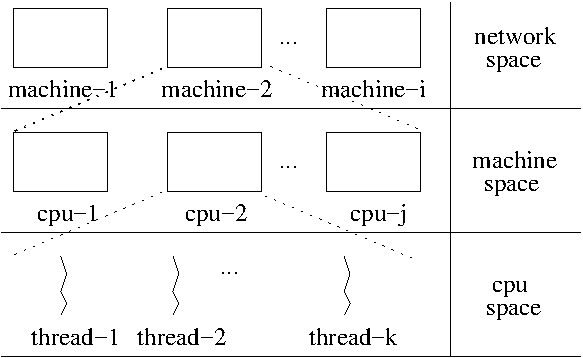
\includegraphics[width=0.35\textwidth]{figs/parallel-levels.pdf}    
  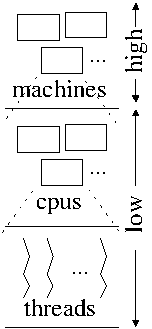
\includegraphics[width=0.08\textwidth]{figs/parallel-levels-short.pdf}  
  \caption{\label{fig:levels}Levels of parallelism.}
  \vspace{-2ex}
\end{wrapfigure}
distribute test execution.  The lowest levels denote parallelism
obtained within a single machine.  These levels are complementary:
the lowest levels leverage the computing power of server
nodes whereas the highest level leverages the aggregate processing
power of a network of machines.
This paper focuses on low-level parallelism, where computation can be
offloaded at different CPUs within a machine and at different threads
within each CPU.  This form of parallelism is enabled through build
systems (spawning processes in different CPUs) and testing frameworks
(spawning threads in one given CPU).  It is important to note that a variety
of testing frameworks provide today support for parallel test
execution (e.g., JUnit~\cite{junit-org}, TestNG~\cite{testng}, and
NUnit~\cite{nunit}) as to benefit from the available power of popular multi-core processors.
In the following, we elaborate relevant features of testing frameworks
and build systems for parallelization.  We focused on Java, Maven, and JUnit but the
discussion can be generalized to other language and tools.

\subsection{Testing Frameworks}
\label{sec:frameworks}

The list below shows the choices to control parallelism within one
Java Virtual Machine (JVM).  These options are offered by the testing
framework (\eg{}, JUnit).

\begin{itemize}
\item
    \textbf{Sequential (\Seq).}~No parallelism is involved.
\item
    \textbf{Sequential classes; parallel methods
      (\SeqClassParMeth).}~This configuration corresponds to running
    test classes sequentially, but running test methods from those
    classes concurrently.
\item
    \textbf{Parallel classes; sequential methods
      (\ParClassSeqMeth{}).}~This configuration corresponds to running
    test classes concurrently, but running test methods sequentially.
\item
    \textbf{Parallel classes; Parallel methods
      (\ParClassParMeth).}~This configuration runs test classes and
    methods concurrently.\Comment{corresponds to the
    combination of \SeqClassParMeth{} and \ParClassSeqMeth{}.  }
\end{itemize}

%% The configuration \Seq{} is a proper fit for short-running test suites
%% since this is the default configuration and the execution provides
%% feedback in an acceptable time. However, for costly suites, it is
%% impractical for developers to wait long-running executions to take
%% action.  In this scenario, the remaining configuration may help to
%% amortize the execution cost depending on how the test suite was
%% designed. For instance,

Notice that an important aspect in deciding which configuration to use
(or in designing new test suites) is the possibility of race
conditions on shared data during execution.  Data sharing can occur,
for example, through state that is reachable from statically-declared variables in
the program or through variables declared within the scope of the test
class or even through resources available on the file system and the network~\cite{luo-etal-fse2014}.  Considering data race avoidance,
configuration \SeqClassParMeth{} is preferable over \ParClassSeqMeth{}
when it is clear that test methods in a class do not manipulate shared
state, which can be challenging to
determine~\cite{bell-etal-esecfse2015}.  Similarly, \ParClassSeqMeth{}
is preferable over \SeqClassParMeth{} when it is clear that several
test methods in a class perform operations involving shared data.
Configuration \ParClassParMeth{} does not restrict scheduling
orderings.  Consequently, it is more likely to manifest data races
during execution. Note that speedups depend on several factors,
including the test suite size and distribution of test methods per
class.

\subsection{Build Systems}
\label{sec:builder}

%% The build system can spawn multiple JVMs, each running on its own OS
%% process on a given CPU and handling a partition of the test set.
Forking OS processes to run test jobs is the basic mechanism of build
systems to obtain parallelism at the machine space (see
Figure~\ref{fig:levels}).  For Java-based build systems, such as Maven
and Ant, this amounts to spawning one JVM, on a given CPU, to handle a
test job and aggregating results when jobs finish.  The list below
shows the choices to control parallelism through the build system
(\eg{}, Maven).

\begin{itemize}
\item
  \textbf{Forked JVMs with sequential methods (\ForkSeq).}~The build
  system spawns multiple JVMs with this configuration, assigning a
  partition of the set of test classes to each JVM.  Test classes and methods
  run sequentially within each JVM.
\item
  \textbf{Forked JVMs with parallel methods (\ForkParMeth).}~With
  this configuration, the build system forks multiple JVMs, as
  \ForkSeq{} does, but it runs test methods concurrently, as
  \SeqClassParMeth{} does.
\end{itemize}

%% In the configuration \ForkSeq{}, each spawned
%% process runs a different test class at time and the builder merges the
%% results from each execution. In the configuration \ForkParMeth{}, the
%% build system forwards settings to the underlying testing framework to
%% enable parallel execution within each process in addition to running
%% test classes on different processes.

Note from the listing that forking can only be combined with
configuration \SeqClassParMeth{} (see Section~\ref{sec:frameworks}) as
Maven made the design choice to only accept one test class at a time
per forked process.  Maven offers an option to reuse JVMs that can be
used to attenuate the potentially high cost of spawning new JVM
processes on every test class (if reuse is enabled) and also to
achieve test isolation (if reuse is disabled).

%% \Mar{$\leftarrow$Are you sure about this?
%%   It seems silly.  Maybe, the rationale is to ``keep design
%%   simple''.}\Jbc{I'm sure. in addition to keep design simple, I feel
%%   like this was initially conceived to run tests in isolation}
%% \Mar{$\leftarrow$confirma?  se sim, pode mostrar isto na
%%   configuracao abaixo?}\Jbc{added...}
%%We are unaware of other build system capable of running multiple
%%classes at time within a forked process.
%%  to
%% define tasks related to the project building and these tasks are
%% performed several plugins.This file
%% contains defintions of tasks, which are implemented by a collection of
%% plugins.
%% \Jbc{falar do surefire e explicar a
%% configuracao ilustrada - Surefire levanta uma JVM por core e cria uma
%% pool de 5 threads em cada JVM para executar testes em paralelo.}
\begin{figure}[h!]
\centering
\scriptsize
\lstset{
  escapeinside={@}{@},
  numbers=none,xleftmargin=1em,frame=none,framexleftmargin=0.5em,
  basicstyle=\ttfamily\scriptsize, boxpos=c, numberstyle=\tiny,
  morekeywords={parallel, threadCount, perCoreThreadCount,
  forkCount, reuseForks},
  deletekeywords={true}
}
\begin{lstlisting}
<plugin>
    <groupId>org.apache.maven.plugins</groupId>
    <artifactId>maven-surefire-plugin</artifactId>
    <configuration>
        <forkCount>1C</forkCount>
        <reuseForks>true</reuseForks>
        <parallel>methods</parallel>
        <threadCount>5</threadCount>
    </configuration>
</plugin>
\end{lstlisting}
  \caption{\label{fig:surefire} Configuration \ForkParMeth{} on
    Maven.}
\vspace{-1ex}  
\end{figure}


\subsubsection*{Example}~Figure~\ref{fig:surefire} shows a
fragment of a Maven configuration file, known as \pomf{}, highlighting
options to run tests using the parallel execution mode \ForkParMeth{}.
Maven implements this feature through its Surefire JUnit test
plugin~\cite{maven-surefire-plugin}.  With this configuration, Maven
forks one JVM per core (\CodeIn{forkCount} parameter) and uses five
threads (\CodeIn{threadCount} parameter) to run test methods
(\CodeIn{parallel} parameter) within each forked JVM.  Maven reuses
created JVMs on subsequent forks when execution of a test class
terminates (\CodeIn{reuseFork} parameter).

%%  LocalWords:  parallelization CPUs JUnit TestNG NUnit multi JVM de
%%  LocalWords:  JVMs falar explicar configuracao ilustrada levanta
%%  LocalWords:  uma por cria cada executar paralelo escapeinside
%%  LocalWords:  xleftmargin framexleftmargin basicstyle boxpos
%%  LocalWords:  numberstyle morekeywords threadCount forkCount
%%  LocalWords:  perCoreThreadCount reuseFork deletekeywords groupId
%%  LocalWords:  artifactId reuseForks
